%%%  Ukázkový text a dokumentace stylu pro text závěrečné (bakalářské a
%%%  diplomové) práce na KI PřF UP v Olomouci
%%%  Copyright (C) 2012 Martin Rotter, <rotter.martinos@gmail.com>
%%%  Copyright (C) 2014 Jan Outrata, <jan.outrata@upol.cz>


%%  Pro získání PDF souboru dokumentu je třeba tento zdrojový text v
%%  LaTeXu přeložit (dvakrát) programem pdfLaTeX.

%%  V případě použití programu BibLaTeX pro tvorbu seznamu literatury
%%  je poté ještě třeba spustit program Biber s parametrem jméno
%%  souboru zdrojového textu bez přípony a následně opět (dvakrát)
%%  přeložit zdrojový text programem pdfLaTeX.

%%  Postup získání Postscriptového souboru je popsán v dokumentaci.


%%  Třída dokumentu implementující styl pro závěrečnou práci. Vybrané
%%  nepovinné parametry (ostatní v dokumentaci):

%%  'master' pro sazbu diplomové práce, jinak se sází bakalářská práce

%%  'field=kód' pro Váš studijní obor, kódy pro diplomovou práci 'uvt'
%%  pro Učitelství výpočetní techniky pro střední školy a 'binf' pro
%%  Bioinformatiku, jinak je výchozí Informatika, a pro bakalářskou
%%  práci 'ainfk' pro Aplikovanou informatiku v kombinované formě,
%%  'inf' pro Informatiku, 'infv' pro Informatiku pro vzdělávání a
%%  'binf' pro Bioinfomatiku, jinak je výchozí Aplikovaná informatika
%%  v prezenční formě

%%  'printversion' pro sazbu verze pro tisk (nebarevné logo a odkazy,
%%  odkazy s uvedením adresy za odkazem, ne odkazy do rejstříku),
%%  jinak verze pro prohlížeč

%%  'biblatex' pro zapnutí podpory pro sazbu bibliografie pomocí
%%  BibLaTeXu, jinak je výchozí sazba v prostředí thebibliography

%%  'language=jazyk' pro jazyk práce, jazyky english pro anglický,
%%  slovak pro slovenský, jinak je výchozí czech pro český

%%  'font=sans' pro bezpatkový font (Iwona Light), jinak výchozí
%%  patkový (Latin Modern)

\documentclass[
%  master,
  field=inf,
%  printversion,
  biblatex,
  language=english,
%  font=sans,
  glossaries,
  theorems=false,
  index
]{kidiplom}

%% Informace pro úvodní strany. V jazyku práce (pokud není v komentáři
%% uvedeno česky) a anglicky. Uveďte všechny, u kterých není v
%% komentáři uvedeno, že jsou volitelné. Při neuvedení se použijí
%% výchozí texty. Text pro jiný než nastavený jazyk práce (nepovinným
%% parametrem language makra \documentclass, výchozí český) se zadává
%% použitím makra s uvedením jazyka jako nepovinného parametru.

%% Název práce, česky a anglicky. Měl by se vysázet na jeden řádek.
\title[czech]{Vizualizace třídicích algoritmů}
\title[english]{Visualization of Sorting Algorithms}

%% Volitelný podnázev práce, česky a anglicky. Měl by se vysázet na
%% jeden řádek. Výchozí je prázdný.
%\subtitle{Ukázkový text a dokumentace stylu v \LaTeX{}u}
%\subtitle[english]{Sample text and documentation of the \LaTeX{} style}

%% Jméno autora práce. Makro nemá nepovinný parametr pro uvedení
%% jazyka.
\author{Mykhailo Klunko}

%% Jméno vedoucího práce (včetně titulů). Makro nemá nepovinný
%% parametr pro uvedení jazyka.
\supervisor{Mgr. Tomáš Kühr, Ph.D.}

%% Volitelný rok odevzdání práce. Výchozí je aktuální (kalendářní)
%% rok. Makro nemá nepovinný parametr pro uvedení jazyka.
%\yearofsubmit{\the\year}

%% Anotace práce, včetně anglické (obvykle překlad z jazyka
%% práce). Jeden odstavec!
\annotation[czech]{Cílem práce bylo vytvořit software pro podporu výuky třídících algoritmů pomocí vizualizace průběhu třídění nejznámějšími algoritmy a jejich variantami. Program byl vytvořen s podporou názorné vizualizaci vybraných algoritmů na zadaném či vygenerovaném vstupním poli a krokování průběhu výpočtu se souběžným zobrazením pseudokódu použitého algoritmu a aktuálních hodnot použitých proměnných.}

\annotation[english]{The main goal of the thesis was to create a learning support software with visualization of the most known sorting algorithms and their variations. The application has to support a graphic visualization of selected algorithms on randomly generated or manually created array, step-by-step execution possibility, pseudocode and current state of variables.}

%% Klíčová slova práce, včetně anglických. Oddělená (obvykle) středníkem.
\keywords[czech]{třídící algoritmus; třídění; vizualizace; program}
\keywords[english]{sorting algorithm; sorting; visualization; software}

%% Volitelná specifikace příloh textu práce, i anglicky. Výchozí je '1
%% CD/DVD'.
%\supplements{jedno kulaté placaté CD/DVD s malou kulatou dírou uprostřed}
%\supplements[english]{one round flat CD/DVD with a small round hole in the middle}

%% Volitelné poděkování. Stručné! Výchozí je prázdné. Makro nemá
%% nepovinný parametr pro uvedení jazyka.
\thanks{I would like to acknowledge my sincere gratitude to my supervisor Mgr. Tomáš Kühr, Ph.D. for his patience and guidance throughout my bachelor thesis. Also, I would like to thank my parents for constant motivation and support from their side. Special thanks go to my friends and colleagues.}

%% Cesta k souboru s bibliografií pro její sazbu pomocí BibLaTeXu
%% (zvolenou nepovinným parametrem biblatex makra
%% \documentclass). Použijte pouze při této sazbě, ne při (výchozí)
%% sazbě v prostředí thebibliography.
\bibliography{bibliografie.bib}
%% Další dodatečné styly (balíky) potřebné pro sazbu vlastního textu
%% práce.
\usepackage{lipsum}
\usepackage{algorithm}
\usepackage{bm}
\usepackage{tikz}
\usetikzlibrary{calc, positioning,fit,intersections}
\usepackage{forest}
\usepackage{caption}

\definecolor{mygreenii}{RGB}{34,162,70}
\definecolor{mygreeni}{RGB}{34,162,70}

\begin{document}
%% Sazba úvodních stran -- titulní, s bibliografickými údaji, s
%% anotací a klíčovými slovy, s poděkováním a prohlášením, s obsahem a
%% se seznamy obrázků, tabulek, vět a zdrojových kódů (pokud jejich
%% sazba není vypnutá).
\maketitle

%% Vlastní text závěrečné práce. Pro povinné závěry, před přílohami,
%% použijte prostředí kiconclusions. Povinná je i příloha s obsahem
%% přiloženého CD/DVD.

%% -------------------------------------------------------------------

\newcommand{\BibLaTeX}{\textsc{Bib}\LaTeX}

%\noindent\textcolor{red}{\LARGE Upozornění: Následující text
%  dokumentace stylu, vyjma přílohy~\ref{sec:ObsahCD}, je rozpracovaná
%  a (značně) neúplná verze!!!}

\section{Introduction}

Nowadays sorting algorithms are widely used in software. For example, if you open file explorer on your PC, you may see files sorted in different ways. Searching in sorted data is more efficient than not sorted. Students of computer science start learning different algorithms in the first year of studies and sorting algorithms are among them.

Since I faced the problems of sorting during the course of algorithm design in the first year of my studies, there is an understanding that the visual representation is a vital part of the studying process. During working on the thesis it was very exciting to learn different techniques of sorting algorithms into the depth.

The main goal of the thesis was to create a program which would serve as a tool for understanding how most known sorting algorithms work. There was an attempt to make the best possible user experience. The demonstration software is made in a user-friendly and easy-to-use style. To gain maximal benefit from learning you can try each sorting algorithm on your own data. 

The text of the thesis describes principles of the most known sorting algorithms which are demonstrated in the computer program. It might be used as a source for learning algorithms by students. Also, the program might be easily used as a demonstration by lecturers and tutors during classes. In addition, there is programmer documentation and user guide to the provided software.

Readers of this text are expected to have some programming experience to know basic data structures such as arrays, lists, trees and understand recursive procedures. Also, knowledge of some simple algorithms and their implementations could be helpful. In order to understand the topic better, knowledge of linear algebra and calculus is involved.

I want to apologize to the reader for possible mistakes and typing errors in this text. Thank you for understanding.

\newpage
\subsection{What is an algorithm?}

Before moving on to the main part of the text which describes algorithms and the software, we need to assure that there is an understanding of the basics. We shall begin with the algorithm definition.

What is an algorithm? How can we define it? We may say simply that an algorithm is a sequence of steps or instructions that solves some kind of problem. Although it may be a bit imprecise because we have not defined what does problem mean and what does instruction mean.

Problem is a kind of task that we need to solve. We are facing different problems every day: finding the fastest route to work or home, etc. However, not all of them are problems that may fit our algorithm definition. A suitable definition of a problem has some limitations: problem should be specified by its inputs and all inputs have to be mapped to some outputs.

Step or instruction is some action that is clear to its executor. In our case, it could be a PC.

To solve a problem means to find a solution for each input.

Here is more precise definition by Thomas Cormen: "Informally, an algorithm is any well-defined computational procedure that takes some value, or set of values, as input and produces some value, or set of values, as output. An algorithm is thus a sequence of computational steps that transform the input into the output." \cite{cormen}
\\\\
\textbf{5 features of an algorithm according to D. Knuth\cite{knuth1}:}
\begin{itemize}
	\item \textit{finiteness} - an algorithm should end in a finite number of steps.
	\item \textit{definiteness} - each step of an algorithm should have precise definition. And it means that for the same inputs we will obtain the same results.
	\item \textit{input} - an algorithm may have inputs, they are taken from some set of objects.
	\item \textit{output} - an algorithm may have outputs which should be in some relation with inputs.
	\item \textit{effectiveness} - we may expect an algorithm to be effective. It means "its operations must all be sufficiently basic that they can in principle be done exactly and in a finite length of time by someone using pencil and paper."\cite{knuth1}
\end{itemize}

\subsection{Types of algorithms}

\subsection{Complexity}

Frequently happen situations when we need to know the performance of some algorithm. There might be a necessity to compare performance of some algorithms, for example. Or we might need to know the time for an algorithm to run with some input. And here we are moving to the concept of the algorithm complexity.

There is a time complexity and a space complexity. In general, complexity gives the amount of time or space needed to run an algorithm. To be more precise: time complexity is a function $f:\mathbb{N}\to\mathbb{N}$ that maps each input to the maximum number of steps for this input needed for an algorithm to complete a task. We will be talking here only about the time complexity and will call it just complexity.

Analyzing algorithms we might want to investigate different sides of the algorithm performance. Usually, it could be a \textit{worst-case analysis} or an \textit{average-case analysis}. The worst-case analysis implies determining the longest running time of all inputs with the same length. In the average-case analysis, we take the average running time of inputs with the same length.

Often complexity of an algorithm is measured on the large inputs. Since complexity is expressed by a polynomial, we might want to have it in a more convenient form. This type of estimation is called an \textit{asymptotic analysis}. Such form takes only the highest order term of the polynomial.

To be more clear, let us have an example. $f(n) = 5n^3 + 10n^2 + 20n + 4$, the highest degree term here is $5n^3$. In some cases we can omit the coefficient 5, now $f$ is asymptotically at most $n^3$.

For such approximation there exists \textbf{O notation}:

\begin{enumerate}
	\item \textit{Asymptotic upper bound}(or $O$). For the function $f(n)$, $O(f(n))$ means that the running time or complexity of an algorithm grows as much as the $f(n)$ but may grow more slowly. It represents a worst-case complexity.
	\item \textit{Asymptotic lower bound}(or $\Omega$). If the complexity of some algorithm is in $\Omega(f(n))$, it means that there exists some large $n$ such that the function $f(n)$ is a lower bound for the algorithm running time. It represents the best-case complexity.
	\item \textit{Asymptotic tight bound}(or $\Theta$). This notation combines both lower and upper bounds. This way, it shows an average-case complexity.
\end{enumerate}

Also, there is a \textit{small-o} notation. It slightly differs from the \textit{Big-O} notation. "Big-O notation says that one function is asymptotically no more than  another. To say that one  function is asymptotically less than another we use small-o notation."\cite{sipser}

\begin{figure}[H]
	\begin{center}
		\begin{tikzpicture}
			\draw[->]  (0,0)coordinate(O) -- (7,0) node[anchor=north] {$n$};
			\draw[->]  (0,0) -- (0,6);
			\draw[domain=0:7,smooth,variable=\x,black,name path=c1] plot ({\x},{0.5*\x+1*sin(\x r)+1})node[right]{$c * g(n)$};
			\draw[domain=0:7,smooth,variable=\x,black,name path=c2] plot ({\x},{0.2*\x+0.5*sin(\x r)+1.5})node[right,black]{$f(n)$};
			\fill[red,name intersections={of=c1 and c2}] (intersection-1) circle (2pt);
			\draw[dashed] (intersection-1) -- (intersection-1|-O) node[below]{$n_0$};

		\end{tikzpicture}
		\caption{$f(n)$ in $O(g(n))$} \label{fig:big-omega}
	\end{center}
\end{figure}

For the asymptotic analysis of an algorithm mostly the worst-case complexity is used. Algorithm is considered for practically solvable if its running time is in $O(n^c)$, $c$ is usually a small constant. 

Here are some complexities (from the slowest to the fastest growing):
\begin{enumerate}
 \item $O(1)$ - constant complexity
 \item $O(\log(n))$ - logarithmic
 \item $O(n)$ - linear
 \item $O(n \log(n))$ - linear-logarithmic
 \item $O(n^2)$ - quadratic
 \item $O(2^n)$ - exponential
 \item $O(n!)$ - factorial
\end{enumerate}

\subsection{Sorting}

As was already said that sorting is used for solving a wide range of problems. It may be used for further searching or, for example, as part of different complex tasks. We were talking about sorting. But what actually sorting is?

Simply said, sorting is a process of rearranging of items, which are possible to compare, in ascending or descending order. In the text we are meaning only ascending order if not stated in a different way.

Ascending order means that items in a sequence are arranged from the smallest to the largest item. On the contrary, descending order means positioning from the largest to the smallest item.
\\\\
Sorting algorithms are divided into two main types:
\begin{enumerate}
	\item \textit{Algorithms of internal sorting} - all the data to sort is stored in the internal memory during the sorting process. 
	\item \textit{Algorithms of external sorting} - all the data to sort is stored outside the internal memory (e.g. on a hard disk) and is loaded to the internal memory by small parts.
\end{enumerate}

Here, in the text, we are talking only about the algorithms of internal sorting. Talking about the algorithms of the internal sorting, here are five main techniques which are usually used\cite{knuth3}:
\begin{enumerate}
	\item \textit{Sorting by Insertion}
	\item \textit{Sorting by Exchanging}
	\item \textit{Sorting by Selection}
	\item \textit{Sorting by Merging}
	\item \textit{Sorting by Distribution}
\end{enumerate}

\newpage
\section{Algorithms}

This section describes algorithms represented in the program.

\subsection{Insertion Sort}
\label{sec:insertion}
Insertion Sort algorithm has a simple idea. Assume an array with items to be sorted. We divide the array into two parts: sorted one and unsorted one. At the beginning sorted part consists of the first element. Then, for each item that we have in the unsorted part, we take element and insert it into the right place among the sorted items.

\begin{figure}[H]
\begin{center}
	
	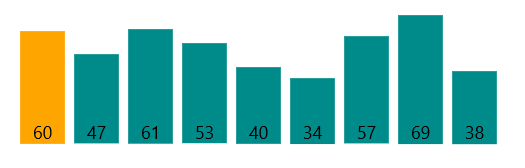
\includegraphics[scale=0.7]{img/Insertion.png}
	\caption{Insertion Sort: sorted and unsorted parts at the beginning}\label{fig:insert}
\end{center}
\end{figure}

In order to insert element into the right place in the sorted part, we compare each item from the unsorted part with each item from the sorted part in the direction from left to right. Comparing continues until smaller or equal element is found or no elements to compare left. After each comparison, if current item in the sorted part is greater, we move that current item one position right. Finally, when the right position is found, we insert an item into the sorted part.

Complexity of Insertion Sort is $\Theta(n^2)$.

\subsection{Selection Sort}
\label{sec:selection}

Selection Sort algorithm is based on the repeated selection. Here we consider finding minimal key from the unsorted part and swapping it with the first unsorted key. As well as in the \hyperref[sec:insertion]{Insertion Sort}, sorted part grows from the beginning of the sequence.

Assume an array of items to sort. At the beginning of the sorting process unsorted part is represented by the whole array. Then, the first item of the unsorted part is set as the smallest key and is compared with the follow-up elements. When smaller item is found, it is set as a new smallest key. After the end of the array is reached the smallest item is swapped with the first element of the unsorted part and it becomes the sorted part of the array. This step is repeated till the array is sorted.

Complexity of this sorting algorithm is $\Theta(n^2)$.

\subsection{Bubble Sort}
\label{sec:bubble}
Bubble Sort is based on the idea of exchanging two adjacent elements if they have wrong order. The algorithm works stepping through all elements from left to right, so the largest elements tend to move or "bubble" to the right. That is why the algorithm is called Bubble Sort.

Now we are going to the details. Let us have an unsorted array. The algorithm does iterations through the unsorted part which is the whole array at the beginning. And with each iteration through the array the range of inspected items is decreased by one till only two elements left. After this two elements are compared and possibly swapped, the array is considered as sorted.

Bubble Sort complexity is $\Theta(n^2)$.

\begin{figure}[H]
\begin{center}
	
	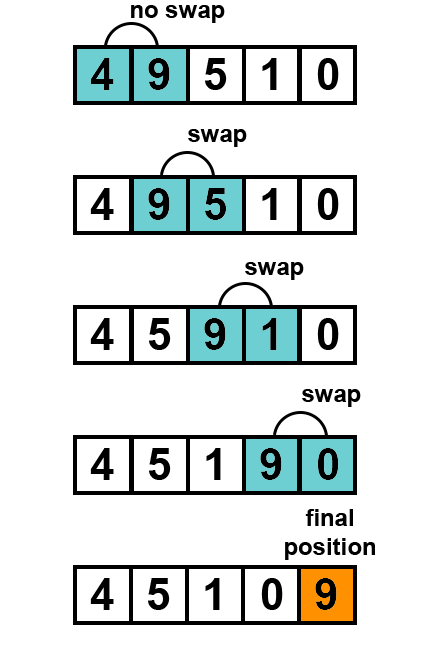
\includegraphics[scale=0.7]{img/Bubblesort.png}
	\caption{Bubble Sort in progress}\label{fig:bubble}
\end{center}
\end{figure}

%add pic of bubblesort in action
\subsection{Cocktail Sort}

Cocktail Sort or also known as Bidirectional Sort. This algorithm similarly to Bubble Sort uses the idea of exchanging unordered adjacent items of array. 

Assume array that needs to be sorted in ascending order. Above we described Bubble Sort and this algorithm has a significant problem. It iterates through array only in one direction. This way, smaller items which are closer to the end of array reach its right positions slowly.

Solution is to make Bubble Sort iterate left-to-right and right-to-left. Cocktail Sort uses two cycles inside a big one:

\begin{enumerate}
 \item Iterate from $a$ to $b$, compare adjacent elements and swap if they are not ordered.
 \item Iterate from $b$ to $a + 1$ same way as in the step $1$
 \item Repeat steps 1. and 2. but with a bit different range from $a = a + 1$ to $b = b - 1$
\end{enumerate}

Cocktail Sort works better than \hyperref[sec:bubble]{Bubble Sort} in some situations, e.g. array is already sorted. However, number of swaps remains the same. This way, worst case complexity remains $\Theta(n^2)$.

\subsection{Quick Sort}

Quick Sort works on the principle "divide and conquer". It recursively applies itself on smaller parts of array until it is not sorted.

Algorithm takes one item at unsorted array or its part, usually it is the leftmost or the rightmost element of array. Then this item also known as pivot is moved to its final position in the array that is should occupy. While determining pivot's position, other elements of array are rearranged the way that no bigger elements on the right and no smaller elements are on the left.

This way, it is enough to apply Quick Sort on each part of array not including pivot until array is not sorted.

\begin{figure}[H]
\begin{center}
	
	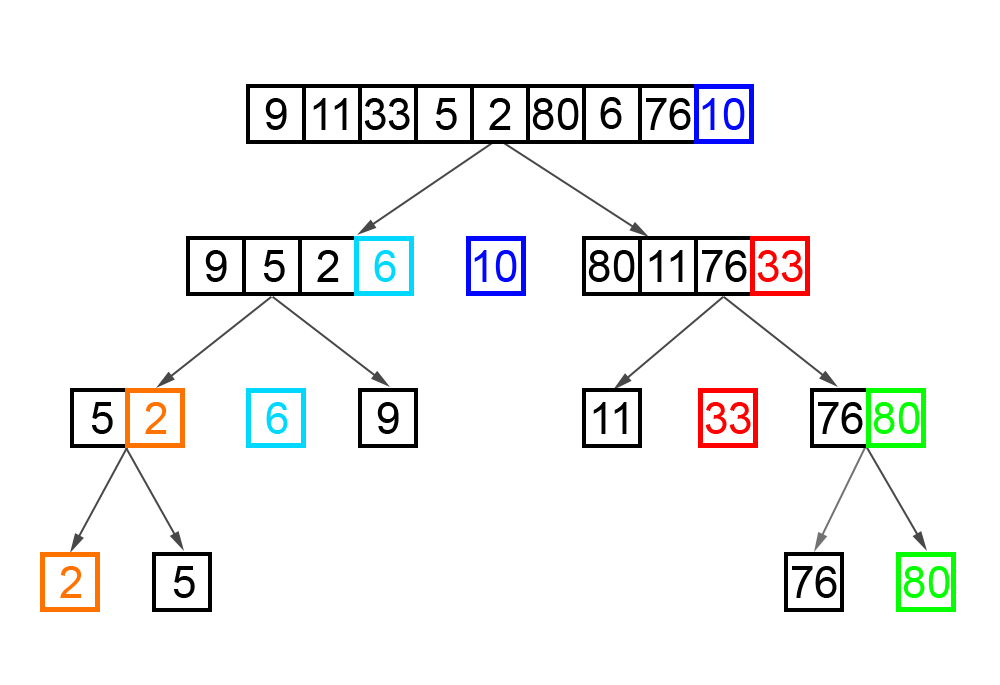
\includegraphics[scale=0.7]{img/Quicksort.png}
	\caption{Quick Sort principle}\label{fig:insert}
\end{center}
\end{figure}

There are several methods of partitioning of array into two parts, here I want to describe one that is demonstrated in the software part of this work.

Firstly, a pivot and index item are selected on the unsorted array or its part. Assume pivot is the last item and index is the first. Next each item of array except pivot is compared with the pivot. If current item is lesser or equal to pivot, it is swapped with the index item, next in order item becomes index. Finally, index and pivot are swapped and this way pivot is on its final position.

Quick Sort is counted as an effective algorithm because its average complexity is $\Theta(n \log n)$. However, when array is maximally unbalanced it may show worst performance. Worst case complexity is $\Theta(n^2)$.

\subsection{Merge Sort}

Merge Sort as well as Quick Sort is an algorithm of type "divide and conquer". The logic of it is simple: recursively divide data into two parts till it becomes indivisible then merge parts back.

Merge procedure itself takes items from each previously divided part one by one, compares them and moves the smallest to the output, repeats previous step.

Merge Sort complexity is $\Theta(n \log n)$

\begin{figure}[H]
\begin{center}
	
	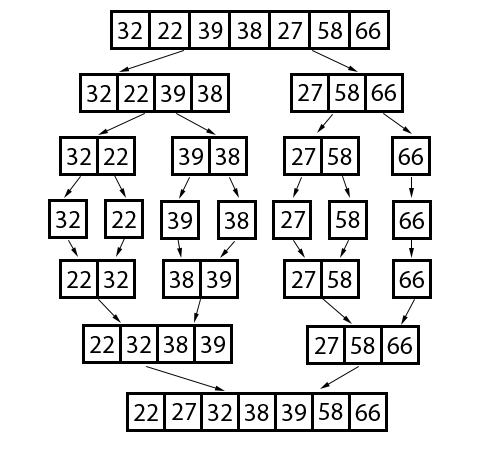
\includegraphics[scale=2.5]{img/Mergesort.png}
	\caption{Merge Sort principle}\label{fig:insert}
\end{center}
\end{figure}

\subsection{Heap Sort}

Heap Sort is a selection based algorithm and it offers another interesting approach to sorting. In comparison with the \hyperref[sec:selection]{Selection Sort} it has optimized selection by using binary heap data structure. 

Binary heap is a complete binary tree; it means that all levels of tree, except the last one, must be completely filled with nodes. Also, this data structure satisfies the \textit{heap condition}: each node key is greater than or equal to its child keys (this heap type is called \textit{max-heap}).

\begin{figure}[H]
\begin{center}
	
	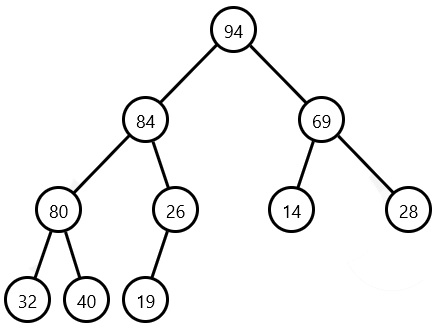
\includegraphics[scale=0.7]{img/Maxheap.png}
	\caption{Max-Heap}\label{fig:maxheap}
\end{center}
\end{figure}

Binary heap may be implemented by simple array. Item at position zero is a root node, items at position one and two are respectively left and right children of the root. From that representation it is easy to find children of each node (if they exist). Assume a node at position $k$ then its left child is at $2k + 1$ and its right child is at $2k + 2$.

\begin{figure}[H]
\begin{center}
	
	
\includegraphics[scale=3]{img/Heapsort.png}
	\caption{Children positions in heap}\label{fig:heapsort}
\end{center}
\end{figure}

\textbf{Heap Sort itself works as follows:}
\begin{enumerate}
 \item \label{itm:step1} Build max-heap
 \item \label{itm:step2} Swap root and the last node, reduce size of heap by one
 \item \label{itm:step3} Build max-heap without the node on a reduced position
 \item Repeat steps \ref{itm:step2} and \ref{itm:step3} until the range of array is one
\end{enumerate}

To build \textit{max-heap} from current node we need to assure that right and left child comprise max-heaps. This way, in the first step procedure for building max-heap is recursively applied for each node that has at least one child from bottom to top.

After each swap of the root node and the node at last considered position last node takes its final place. This way it joins the sorted part of array.

Worst and average case complexity of Heap Sort are both $\bm{\Theta(n \log(n))}$.

\subsection{Counting Sort} \label{sec:counting}

Counting Sort is usually used for sorting integer keys in the range from $0$ to $k$. Algorithm is based on counting keys of distinct values. Final positions of keys are calculated from the previous computations. It means that the position of some key $x$ depends on the count of keys that are less than $x$.

For better understanding let us have an example. Assume we have integers in the range from $0$ to $k$ and an empty output array. For this range we create helping array that will keep counters for each number from the range. Then all counters from the helping array are set to $0$. To obtain final positions for items to be sorted we need to make further computations.

Firstly, for each element from the initial array we increase the respective counter which is determined from the element value. That means value of the element is its counter position in the helping array. Secondly, we need to sum each counter with previous. Finally, for each item from the initial array the respective counter is decreased by one and the value of counter now is the final position, we move item to the output array.

Worst case complexity for Counting Sort is $\Theta(k + n)$, where $k$ is number of items in range and $n$ is size of array to be sorted.

\subsection{Radix Sort}

The Radix sorting algorithm is based on the idea of using separate digits to determine final number positions. It works with the help of some stable sorting algorithm, it can be for example \hyperref[sec:counting]{Counting Sort}, taking digits one by one from least significant to most significant.

For better understanding let us go to the details. Assume the array of integers. Let $d$ be the number of digits of the largest item from the array. If there are numbers from the array that have less digits than the $d$ is, then insufficient digits are counted as digits with zero values.

This way, for each digit from least significant to most we sort the input array according to the current digit. Here we use \hyperref[sec:counting]{Counting Sort} or another stable algorithm.

\begin{figure}[H]
\begin{center}
	
	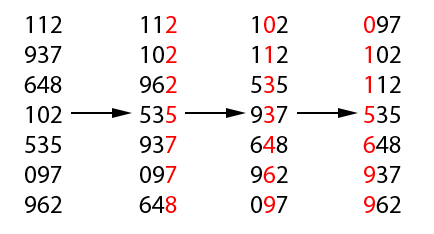
\includegraphics[scale=2]{img/Radixsort.png}
	\caption{Radix Sort example}\label{fig:radixsort}
\end{center}
\end{figure}

\subsection{Bucket Sort}

Bucket Sort as well as \hyperref[sec:counting]{Counting Sort} requires to know range of sorted data in advance. It is suitable when data is uniformly distributed over the range.

At the beginning algorithm creates $n$ intervals of same size. For each interval there is created a dynamic structure which will held items from the input. This dynamic structures are called buckets.

Firstly, Bucket Sort distributes data to buckets. Then, there is need to sort each non-empty bucket. This task can be done by using, for example, \hyperref[sec:insertion]{Insertion Sort}. Finally, items from each bucket one by one are moved to the output array.

\begin{figure}[H]
\begin{center}
	
	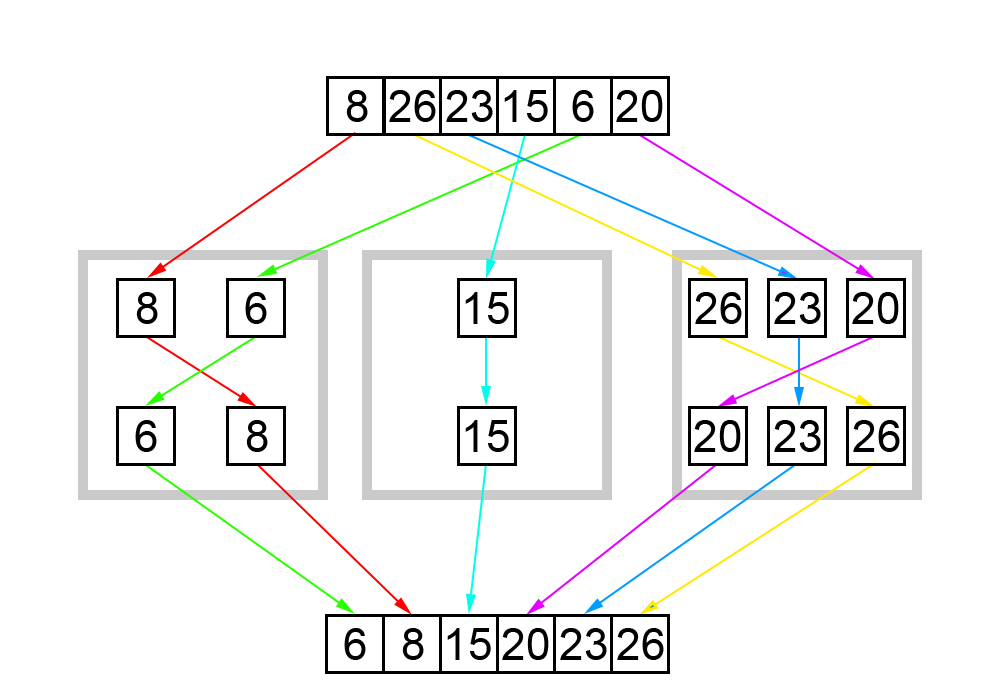
\includegraphics[scale=0.5]{img/Bucketsort.png}
	\caption{Bucket Sort}\label{fig:radixsort}
\end{center}
\end{figure}

\newpage
\section{Documentation}

This section describes the structure of the program and some useful topics from the programmer's side. 

\subsection{Used technologies}

Nowadays exist a lot of programming languages, libraries, frameworks. On the one hand, a software developer has a wide choice. On the other hand, here comes up a new problem to make the right choice which should fit the best to the current task.

The main programming language of the thesis software is Java. To be more precise, Java Platform, Standard Edition 8. Java is a cross-platform, object-oriented language. Its motto is "write once, run anywhere". It means that compiled java application runs on all platforms, that are supported by Java. Java applications are compiled to the kind of bytecode and may be running on the \Gls{JVM} regardless of the platform. 

\begin{figure}[H]
\begin{center}
	
	
\includegraphics[scale=0.2]{img/java_logo.png}
	\caption{Java}\label{fig:java}
\end{center}
\end{figure}

As for the visual side of the application, Java provides a good JavaFX library which is enough for the purpose. Here JavaFX was used both for the user interface and algorithms visualization. Also, JavaFX provides the possibility of using \Gls{CSS}. The visualization software uses \Gls{CSS} for styling some elements of the user interface.

The project was created and developed in the NetBeans IDE, although you may use other IDEs that support importing the NetBeans projects. It was developed under the Windows operating system and was tested with different screens and on the macOS. A version control system Git in connection with the GitHub was used. All the work on the project you may track on \href{https://github.com/klnmi97/Sorting-Visualization}{the GitHub website}.

\newpage
\subsection{Structure}

Program source codes are structured into packages:
\begin{figure}[H]
	\begin{flushleft}
		\begin{forest}
			for tree={
    		font=\sffamily,
    		text=white,
    		text width=3.5cm,
    		minimum height=0.5cm,
    		if level=0
    		  {fill=mygreenii}
    		  {fill=mygreeni},
    		rounded corners=4pt,
    		grow'=0,
    		child anchor=west,
    		parent anchor=south,
    		anchor=west,
    		calign=first,
    		edge={mygreenii,rounded corners,line width=1pt},
    		edge path={
    		  \noexpand\path [draw, \forestoption{edge}]
    		  (!u.south west) +(7.5pt,0) |- (.child anchor)\forestoption{edge label};
		    },
    		before typesetting nodes={
      		if n=1
        		{insert before={[,phantom]}}
        		{}
    		},
    		fit=band,
    		s sep=10pt,
    		before computing xy={l=15pt},
  		}
		[sortingvisualization
		  [Constants]
  		  [Controllers]
		  [Data]
		  [Enums]
		  [NodeControllers]
		  [UI]
		  [Utilities]
		  [Algorithms]
		]
		\end{forest}
		%\captionsetup{justification=raggedright, singlelinecheck=false}
		%\caption{Project structure}\label{fig:structure}
	\end{flushleft}
\end{figure}

Each package contains certain classes, which are grouped by the purpose of use. Next subsections contain some general descriptions of the classes from packages. 
\subsubsection{A root package}
The root package contains only one class. It is MainUI.java. This class serves as the main class which starts the application. Although JavaFX provides the possibility of using XML-based language for creating a user interface, here it is not used. 

The MainUI class defines main user interface elements and does the instantiating of controllers.

\subsubsection{Constants, Data and Enum packages}
All this three packages work with data and data structures although a bit differently.

Constants package has only an eponymous class. This class contains final static variables that are used as default values in the program.

Data package contains classes which serve as definitions for data objects. BindingData class instance holds data for control buttons bindings. Results class defines object that is used for transferring results from the input dialog.

Enum package contains one definition of the enum class. Algorithm enum defines list of algorithms that are visualized in the program. For example, a list with algorithm names in the main window is generated from this enum.

\newpage
\section{User Guide}

\begin{figure}[H]
\begin{center}
	
	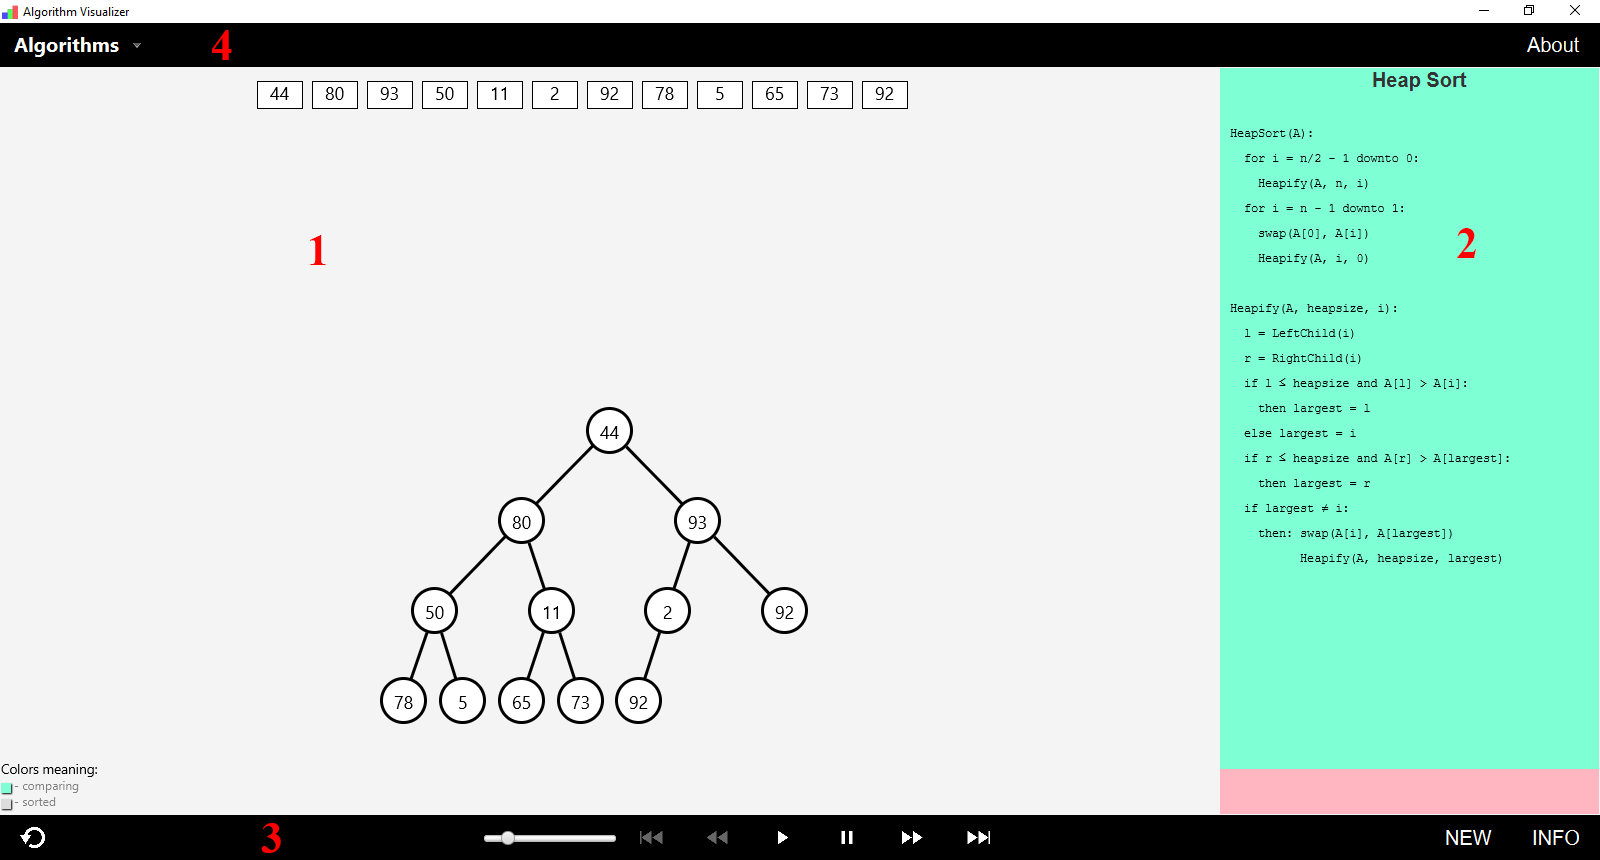
\includegraphics[scale=0.34]{img/UI.png}
	\caption{Main window}\label{fig:ui}
\end{center}
\end{figure}

%% Závěry práce. V jazyce práce a anglicky. Text pro jiný než
%% nastavený jazyk práce (nepovinným parametrem language makra
%% \documentclass, výchozí český) se zadává použitím makra s uvedením
%% jazyka jako nepovinného parametru.
\begin{kiconclusions}
Závěr práce v \uv{českém} jazyce.
\end{kiconclusions}

\begin{kiconclusions}[english]
Thesis conclusions in \uv{English}.
\end{kiconclusions}

%% Přílohy obsahu textu práce, za makrem \appendix.
\appendix

\section{První příloha}
Text první přílohy

\section{Druhá příloha}
Text druhé přílohy

%% Obsah přiloženého CD/DVD. Poslední příloha. Upravte podle vlastní
%% práce!
\section{Obsah přiloženého CD/DVD} \label{sec:ObsahCD}

Na samotném konci textu práce je uveden stručný popis obsahu
přiloženého CD/DVD, tj.~jeho závazné adresářové struktury, důležitých
souborů apod.

\begin{description}

\item[\texttt{bin/}] \hfill \\
  Instalátor \textsc{Instalator} programu, popř.~program
  \textsc{Program}, spustitelné přímo z~CD/DVD. / Kompletní adresářová
  struktura webové aplikace \textsc{Webovka} (v~ZIP archivu) pro
  zkopírování na webový server. Adresář obsahuje i~všechny runtime
  knihovny a~další soubory potřebné pro bezproblémový běh instalátoru
  a~programu z~CD/DVD / pro bezproblémový provoz webové aplikace na
  webovém serveru.

\item[\texttt{doc/}] \hfill \\
  Text práce ve formátu PDF, vytvořený s~použitím závazného stylu KI
  PřF UP v~Olomouci pro závěrečné práce, včetně všech příloh,
  a~všechny soubory potřebné pro bezproblémové vygenerování PDF
  dokumentu textu (v~ZIP archivu), tj.~zdrojový text textu, vložené
  obrázky, apod.

\item[\texttt{src/}] \hfill \\
  Kompletní zdrojové texty programu \textsc{Program} / webové aplikace
  \textsc{Webovka} se všemi potřebnými (příp.~převzatými) zdrojovými
  texty, knihovnami a~dalšími soubory potřebnými pro bezproblémové
  vytvoření spustitelných verzí programu / adresářové struktury pro
  zkopírování na webový server.

\item[\texttt{readme.txt}] \hfill \\
  Instrukce pro instalaci a~spuštění programu \textsc{Program}, včetně
  všech požadavků pro jeho bezproblémový provoz. / Instrukce pro
  nasazení webové aplikace \textsc{Webovka} na webový server, včetně
  všech požadavků pro její bezproblémový provoz, a~webová adresa, na
  které je aplikace nasazena pro účel testování při tvorbě posudků
  práce a~pro účel obhajoby práce.

\end{description}

Navíc CD/DVD obsahuje:

\begin{description}

\item[\texttt{data/}] \hfill \\
  Ukázková a~testovací data použitá v~práci a~pro potřeby testování
  práce při tvorbě posudků a~obhajoby práce.

\item[\texttt{install/}] \hfill \\
  Instalátory aplikací, runtime knihoven a~jiných souborů potřebných
  pro provoz programu \textsc{Program} / webové aplikace
  \textsc{Webovka}, které nejsou standardní součástí operačního
  systému určeného pro běh programu / provoz webové aplikace.

\item[\texttt{literature/}] \hfill \\
  Vybrané položky bibliografie, příp.~jiná užitečná literatura
  vztahující se k~práci.

\end{description}

U~veškerých cizích převzatých materiálů obsažených na CD/DVD jejich
zahrnutí dovolují podmínky pro jejich šíření nebo přiložený souhlas
držitele copyrightu. Pro všechny použité (a~citované) materiály,
u~kterých toto není splněno a~nejsou tak obsaženy na CD/DVD, je uveden
jejich zdroj (např.~webová adresa) v~bibliografii nebo textu práce
nebo v souboru \texttt{readme.txt}.

%% -------------------------------------------------------------------

%% Sazba volitelného seznamu zkratek, za přílohami.
\printglossary


%% Sazba povinné bibliografie, za přílohami (případně i za seznamem
%% zkratek). Při použití BibLaTeXu použijte makro
%% \printbibliography. jinak prostředí thebibliography. Ne obojí!

%% Sazba i v textu necitovaných zdrojů, při použití
%% BibLaTeXu. Volitelné.
\nocite{*}
%% Vlastní sazba bibliografie při použití BibLaTeXu.
\printbibliography

%% Bibliografie, včetně sazby, při nepoužití BibLaTeXu.
% \begin{thebibliography}{9}
%\bibitem{kniha2} \uppercase{Hawke}, Paul. NanoHttpd: Light-weight HTTP server designed for embedding in other applications. GitHub [online]. 2014-05-12. [cit. 2014-12-06]. Dostupné z: \url{https://github.com/NanoHttpd/nanohttpd}
%
%\bibitem{jeske13} \uppercase{Jeske}, David; \uppercase{Novák}, Josef. Simple HTTP Server in \csharp: Threaded synchronous HTTP Server abstract class, to respond to HTTP requests. CodeProject: For those who code [online]. 2014-05-24. [cit. 2014-12-06]. Dostupné z: \url{http://www.codeproject.com/Articles/137979/Simple-HTTP-Server-in-C}
%
%\bibitem{uzis2012} \uppercase{ÚSTAV ZDRAVOTNICKÝCH INFORMACÍ A STATISTIKY ČR}. Lékaři, zubní lékaři a farmaceuti 2012 [online]. Praha 2, Palackého náměstí 4: Ústav zdravotnických informací a statistiky ČR, 2012 [cit. 2014-12-06]. ISBN 978-80-7472-089-5. Dostupné z: \url{http://www.uzis.cz/publikace/lekari-zubni-lekari-farmaceuti-2012}
% \end{thebibliography}

%% Sazba volitelného rejstříku, za bibliografií.
%\printindex

\end{document}
